\section{Temporal Graph Model}
\label{sec:tga}

\begin{figure}[t]
\centering
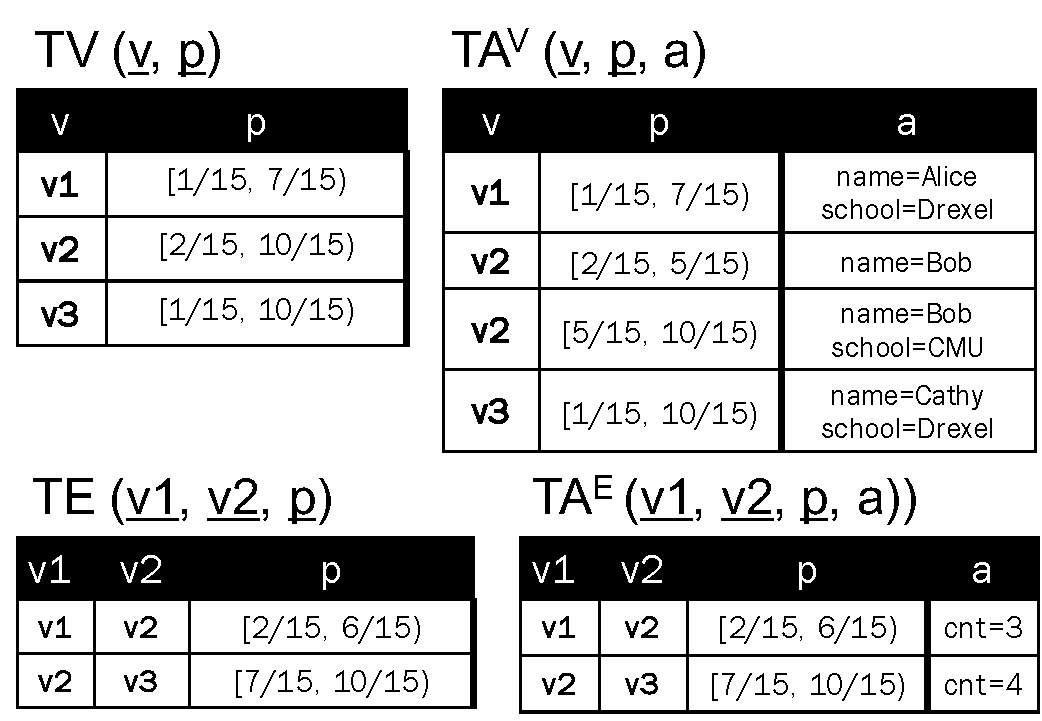
\includegraphics[width=2.5in]{figs/T1_rel.pdf}
\vspace{-0.2cm}
\caption{\tg \insql{T1}.}
\vspace{-0.5cm}
\label{fig:tg_rel}
\end{figure}

Our data model is based on the temporal relational model, and our
algebra corresponds to temporal relational algebra, but is designed
specifically for evolving graphs.  

{\bf Data model.}  In~\cite{PortalarXiv2016} we proposed an evolving
graph model \tg based on valid-time temporal relations with point
semantics. An example is shown in Figure~\ref{fig:tg_rel}.  A \tg
consists of two temporal relations, \insql{V} and \insql{E}, that
represent the vertices and edges of the graph with their corresponding
validity periods expressed by intervals.  Optionally, temporal
relations \insql{VA} and \insql{EA} represent vertex and edge
attributes using the property model.

A \tg represents a single graph, e.g., the Web.\eat{, and models
  evolution of its topology and of vertex and edge attributes.}  A
snapshot of a \tg is the state of the relations at any time point.
\tg relations are coalesced~\cite{DBLP:conf/vldb/BohlenSS96} --- each
fact (existence of a vertex or edge, or an assignment of a value to a
vertex or edge attribute) is represented exactly once for each time
period of maximal length during which it holds.  Referential integrity
holds on \insql{E} w.r.t. \insql{V}, guaranteeing that edges only
exist if their end points exist at the same time, on \insql{VA}
w.r.t. \insql{V}, and on \insql{EA} w.r.t. \insql{E}.

{\bf Operations.} In~\cite{PortalarXiv2016} we proposed a temporal
graph algebra \tga.  The algebra is compositional: operators take a
\tg or a pair of \tgs as input, and output a \tg.  \tga semantics can
be expressed as a sequence of temporal relational algebra expressions,
guaranteeing snapshot reducibility and extended snapshot
reducibility~\cite{DBLP:reference/db/Bohlen092} --- two properties
appropriate for a point-based temporal data model.  The operations of
\tga include slice, map, selection, aggregation, node creation, edge
creation, and binary operations union, intersection, and difference.
We study the expressiveness of \tga in~\cite{PortalarXiv2016} and show
completeness w.r.t. temporal relational algebra.  We also support
\eat{Pregel-style}graph analytics that are logically executed on each
snapshot.

In the next section, we explain the operations of TGA through
examples, and refer the reader to~\cite{PortalarXiv2016} for
additional details.  The next section also serves to introduce the
syntax of \ql, a declarative language, whose queries are rewritten by
the \sys system into sequence of \tga operations.  \ql is being
presented here for the first time.
